\section*{Appendices}
\addcontentsline{toc}{section}{Appendices}
\renewcommand{\thesubsection}{\Alph{subsection}}

\subsection{Profiling Framework}
\label{appendix:profiling}

We implemented a custom profling framework for PyTorch to collect data for detailed runtime 
and memory usage analysis. Our profiler contains three components:

\begin{enumerate}
    \item \textit{Resource monitor thread}: Runs in parallel to the data parallel training 
    processes and tracks CPU memory usage, as well as memory usage on each GPU. The monitor 
    takes snapshot at a configurable time interval (2 seconds for all our runs).
    \item \textit{Phase clocking component}: Tracks runtime of all phases during each training 
    step, as well as total epoch time. The phases include time spend on fetching data from 
    the dataloader, forward pass, and backward pass. All phase times are tracking through clocks 
    which are activated when the training scripts enters a specific phase and deactivated when 
    it leaves the phase.
    \item \textit{PyTorch internal memory tracker}: Tracks allocated and reserved memory from 
    PyTorch directly. This allows the profiler to detect how much GPU memory is used only for
    tensors and not any other components of the framework.
\end{enumerate}


The profiler is implemented as part of the OCP codebase. The implementation of each component 
is located in the tracking package\footnote{\url{https://github.com/TUM-DI-Lab-Graph-Scaling/ocp/tree/main/ocpmodels/tracking}}.

Our profiler is not an alternative to the official PyTorch profiler, but rather a complementary 
module to gather data on long running experiments. For shorter experiments, which just run over 
the span of a few training steps, the PyTorch profilier offers far more detailed data collection 
and better visualization support through a Tensorboard plugin.


\newpage

\subsection{Per-Experiment Memory Usage}

The figures below show memory utilization for 
CUDA tensors averaged over all GPUs over time. 
Allocated memory is \textcolor{tum-dark-blue}{blue},
while reserved memory is \textcolor{tum-orange}{orange}.

\begin{figure}[H]

    \centering

    \begin{subfigure}[t]{0.45\textwidth}
        \centering
        \includegraphics[width=\textwidth]{evaluation/gemnet/s2ef/cuda_memory/S0/averaged.pdf}
    \end{subfigure}%
    ~
    \begin{subfigure}[t]{0.45\textwidth}
        \centering
        \includegraphics[width=\textwidth]{evaluation/gemnet/s2ef/cuda_memory/S0+fp16/averaged.pdf}
    \end{subfigure}

    \begin{subfigure}[t]{0.45\textwidth}
        \centering
        \includegraphics[width=\textwidth]{evaluation/gemnet/s2ef/cuda_memory/S1/averaged.pdf}
    \end{subfigure}%
    ~
    \begin{subfigure}[t]{0.45\textwidth}
        \centering
        \includegraphics[width=\textwidth]{evaluation/gemnet/s2ef/cuda_memory/S1+OC/averaged.pdf}
    \end{subfigure}

    \begin{subfigure}[t]{0.45\textwidth}
        \centering
        \includegraphics[width=\textwidth]{evaluation/gemnet/s2ef/cuda_memory/S2+OC/averaged.pdf}
    \end{subfigure}%
    ~
    \begin{subfigure}[t]{0.45\textwidth}
        \centering
        \includegraphics[width=\textwidth]{evaluation/gemnet/s2ef/cuda_memory/S2+OO+OC/averaged.pdf}
    \end{subfigure}

    \begin{subfigure}[t]{0.45\textwidth}
        \centering
        \includegraphics[width=\textwidth]{evaluation/gemnet/s2ef/cuda_memory/S3+OC/averaged.pdf}
    \end{subfigure}%
    ~
    \begin{subfigure}[t]{0.45\textwidth}
        \centering
        \includegraphics[width=\textwidth]{evaluation/gemnet/s2ef/cuda_memory/S3+PO+OO+OC/averaged.pdf}
    \end{subfigure}

    \caption{GPU memory consumption for GemNet on the S2EF task.}
    
\end{figure}

\begin{figure}[H]

    \centering

    \begin{subfigure}[t]{0.45\textwidth}
        \centering
        \includegraphics[width=\textwidth]{evaluation/gemnet/is2re/cuda_memory/S0/averaged.pdf}
    \end{subfigure}%
    ~
    \begin{subfigure}[t]{0.45\textwidth}
        \centering
        \includegraphics[width=\textwidth]{evaluation/gemnet/is2re/cuda_memory/S0+fp16/averaged.pdf}
    \end{subfigure}

    \begin{subfigure}[t]{0.45\textwidth}
        \centering
        \includegraphics[width=\textwidth]{evaluation/gemnet/is2re/cuda_memory/S1/averaged.pdf}
    \end{subfigure}%
    ~
    \begin{subfigure}[t]{0.45\textwidth}
        \centering
        \includegraphics[width=\textwidth]{evaluation/gemnet/is2re/cuda_memory/S1+OC/averaged.pdf}
    \end{subfigure}

    \begin{subfigure}[t]{0.45\textwidth}
        \centering
        \includegraphics[width=\textwidth]{evaluation/gemnet/is2re/cuda_memory/S2+OC/averaged.pdf}
    \end{subfigure}%
    ~
    \begin{subfigure}[t]{0.45\textwidth}
        \centering
        \includegraphics[width=\textwidth]{evaluation/gemnet/is2re/cuda_memory/S2+OO+OC/averaged.pdf}
    \end{subfigure}

    \begin{subfigure}[t]{0.45\textwidth}
        \centering
        \includegraphics[width=\textwidth]{evaluation/gemnet/is2re/cuda_memory/S3+OC/averaged.pdf}
    \end{subfigure}%
    ~
    \begin{subfigure}[t]{0.45\textwidth}
        \centering
        \includegraphics[width=\textwidth]{evaluation/gemnet/is2re/cuda_memory/S3+PO+OO+OC/averaged.pdf}
    \end{subfigure}

    \caption{GPU memory consumption for GemNet on the IS2RE task.}
    
\end{figure}

\begin{figure}[H]

    \centering

    \begin{subfigure}[t]{0.45\textwidth}
        \centering
        \includegraphics[width=\textwidth]{evaluation/dimenet/s2ef/cuda_memory/S0/averaged.pdf}
    \end{subfigure}%
    ~
    \begin{subfigure}[t]{0.45\textwidth}
        \centering
        \includegraphics[width=\textwidth]{evaluation/dimenet/s2ef/cuda_memory/S0+fp16/averaged.pdf}
    \end{subfigure}

    \begin{subfigure}[t]{0.45\textwidth}
        \centering
        \includegraphics[width=\textwidth]{evaluation/dimenet/s2ef/cuda_memory/S1/averaged.pdf}
    \end{subfigure}%
    ~
    \begin{subfigure}[t]{0.45\textwidth}
        \centering
        \includegraphics[width=\textwidth]{evaluation/dimenet/s2ef/cuda_memory/S1+OC/averaged.pdf}
    \end{subfigure}

    \begin{subfigure}[t]{0.45\textwidth}
        \centering
        \includegraphics[width=\textwidth]{evaluation/dimenet/s2ef/cuda_memory/S3+OC/averaged.pdf}
    \end{subfigure}%
    ~
    \begin{subfigure}[t]{0.45\textwidth}
        \centering
        \includegraphics[width=\textwidth]{evaluation/dimenet/s2ef/cuda_memory/S3+PO+OO+OC/averaged.pdf}
    \end{subfigure}

    \caption{GPU memory consumption for DimeNet++ on the S2EF task.}
    
\end{figure}

\begin{figure}[H]

    \centering

    \begin{subfigure}[t]{0.45\textwidth}
        \centering
        \includegraphics[width=\textwidth]{evaluation/dimenet/is2re/cuda_memory/S0/averaged.pdf}
    \end{subfigure}%
    ~
    \begin{subfigure}[t]{0.45\textwidth}
        \centering
        \includegraphics[width=\textwidth]{evaluation/dimenet/is2re/cuda_memory/S0+fp16/averaged.pdf}
    \end{subfigure}

    \begin{subfigure}[t]{0.45\textwidth}
        \centering
        \includegraphics[width=\textwidth]{evaluation/dimenet/is2re/cuda_memory/S1/averaged.pdf}
    \end{subfigure}%
    ~
    \begin{subfigure}[t]{0.45\textwidth}
        \centering
        \includegraphics[width=\textwidth]{evaluation/dimenet/is2re/cuda_memory/S1+OC/averaged.pdf}
    \end{subfigure}

    \begin{subfigure}[t]{0.45\textwidth}
        \centering
        \includegraphics[width=\textwidth]{evaluation/dimenet/is2re/cuda_memory/S2+OC/averaged.pdf}
    \end{subfigure}%
    ~
    \begin{subfigure}[t]{0.45\textwidth}
        \centering
        \includegraphics[width=\textwidth]{evaluation/dimenet/is2re/cuda_memory/S2+OO+OC/averaged.pdf}
    \end{subfigure}

    \begin{subfigure}[t]{0.45\textwidth}
        \centering
        \includegraphics[width=\textwidth]{evaluation/dimenet/is2re/cuda_memory/S3+OC/averaged.pdf}
    \end{subfigure}%
    ~
    \begin{subfigure}[t]{0.45\textwidth}
        \centering
        \includegraphics[width=\textwidth]{evaluation/dimenet/is2re/cuda_memory/S3+PO+OO+OC/averaged.pdf}
    \end{subfigure}

    \caption{GPU memory consumption for DimeNet++ on the IS2RE task.}
    
\end{figure}